While Model 1 works well predicting the next input digit given the current one, it is limited to working over the entire dataset to first train the GSN and then again to train the regression step (repeating until convergence). Sequential data, however, often requires an online learning method when the entire dataset is not available and must be collected sequentially, while both training and providing predictions as data arrives.

\section{Online learning with real-sequenced data }
The GSNs of Model 1 can be learned in a quasi-online manner: for each sequential group of inputs, perform a GSN training update after \(k\) walkbacks, and then update the regression parameters. However, when updating on an individual input level, these sequential GSNs converge slowly and can get stuck in bad configurations due to the regression step (which is simple linear regression) being trained on a not-yet-useful hidden representation of the complex input data. If the regression step is trained poorly, it affects the remaining GSN parameter training steps by providing bad sequential predictions for the GSN to attempt to reconstruct.

The main claim for Model 2 is that GSNs can learn a complex hidden representation \(H\) that encodes sequences inherent to the input data. Instead of using Gibbs sampling to generate the artificial time series, a GSN can use the real time sequence of the input data to train its parameters with respect to the predicted reconstruction of the next input in the sequence. The GSN becomes a generative sequence prediction model rather than a generative data distribution model. This approach is not without drawbacks - the GSN loses its ability to utilize the walkback training principle for creating robust representations by actively seeking out spurious modes in the model. However, this drawback is mitigated with more input data.  Further, the GSN loses the ability to mix between modes of the input space. Instead, it mixes between modes of the sequence space - learning to transition to the next most likely input given the current and previous data.


\section{Algorithm}

Currently, GSNs use tied weights between layers to make backpropagation easier. However, this approach prohibits the hidden representation from being able to encode sequences. The online learning method must untie these weights, which makes training more difficult.

\begin{algorithm}[h!]
	\KwIn{training data \(X\) in sequential order, \(N\) layers, \(k \geq 2*N\) predictions}
	Initialize GSN parameters \(\Theta_{GSN} = \) \{List(weights from one layer to the next higher), List(weights from one layer to the next lower), List(bias for layer))\}\;
	\For{input data \(x\) received}{
		 Sample from GSN predicted \(x'\) to create a list of the next \(k\) predicted inputs\;
		Store these predictions in a memory buffer array of lists\;
		Use the current input \(x\) to train GSN parameters with respect to the list of predicted \(x'\) through backpropagation\;
	}
	\caption{ Model 2 Online Algorithm }
\end{algorithm}

\section{Results}

Using the same general training parameters with regards to noise, learning rate, annealing, momentum, epochs, hidden layers, and activation as Model 1, Model 2 performs similarly with regards to binary cross-entropy as Model 1 on the artificially sequenced MNIST dataset. For the next immediate predicted number, it achieved a binary cross-entropy of 0.2318.  For the predicted number six iterations ahead, it achieved a binary cross-entropy of 0.2268. This cross-entropy is lower because six iterations ahead can utilize higher layers of representation in the GSN due to the way the computational graph is formed.

Even though cross-entropy is similar to Model 1, reconstruction images paint a different picture. Due to untied weights taking longer to train, the next predicted digits looks less refined than the averages produced from Model 1 over the same number of iterations. However, as the number of predictions ahead increases, the digits begin to look more like the averages. This could be explained by further predictions ahead utilizing the higher layers of representation based on the way the computational graph is formed.

\begin{figure}[h!]
  \centering
    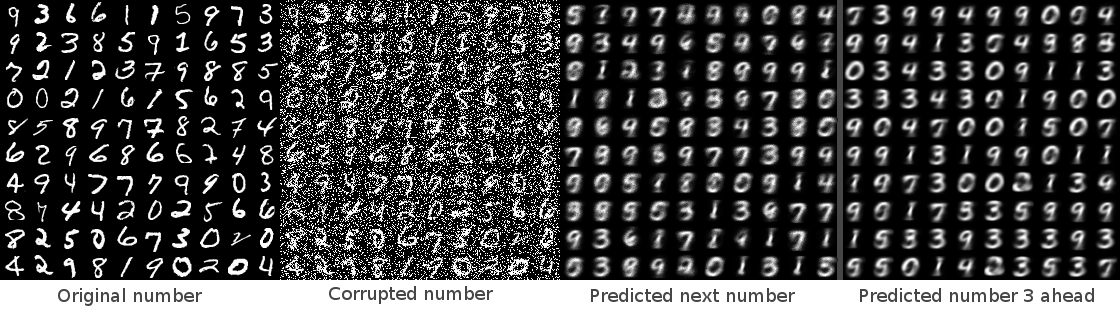
\includegraphics[width=1.0\textwidth]{story2_reconstruction}
\caption{Model 2 reconstruction of predicted next digits and predicted digits 3 iterations ahead after 300 iterations.}
\end{figure}

Learning with untied weights is much slower, but still provides evidence that the hidden layers themselves can learn useful representations for complex input sequences. Looking at the generated samples after 300 training iterations, mixing between sequential modes is evident as the samples appear to be generated in the same 0-9 order as the sequenced data:
\begin{figure}[h!]
  \centering
    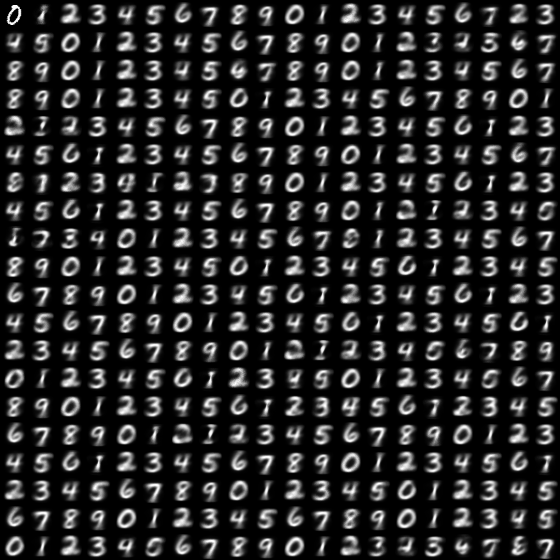
\includegraphics[width=.8\textwidth]{story2_samples_300}
\caption{Model 2 sampling after 300 iterations.}
\end{figure}


\section{Extending the walkback procedure to sequenced inputs}

This online model loses the ability to use walkback training to reduce spurious modes. However, walkback could theoretically be generalized to the sequential case by sampling from possible variations of past hidden representations that could lead to the current input. Intuitively, this idea comes from the method of explaining current inputs with imperfect memory recall of past inputs. By sampling from the representation layer repeatedly, a series of potentially viable past representations that lead to the current input are created and used to train GSN parameters leading to the current input. This method uses past inputs as context to create viable variations of sequences in the representation space, which in turn acts to create more robust mixing between the modes in the sequence space.

The general process for creating sequential walkbacks described here is as follows:
\begin{algorithm}[h!]
	\For{k walkbacks}{
		Given input \(x\), take a backward step with the GSN using transposed weights and negated bias to create the previous hidden representation \(H\)\;
		Sample from the hidden representation \(H\) to form \(H'\)\;
		Take a forward step with the GSN using \(H'\) to create \(x'\)\;
		Use this \((x', x)\) pair as a training example for the GSN parameters\;
	}
	\caption{ Walkbacks for sequential input }
\end{algorithm}
